\documentclass[UTF8, 12pt]{article}
\usepackage{ctex}
\usepackage[utf8]{inputenc}
\usepackage{amsmath}
\usepackage[margin=1in]{geometry}
\usepackage{graphicx}
\usepackage[colorlinks=true, linkcolor=red, urlcolor=blue]{hyperref}
\usepackage{xcolor}
\usepackage{tikz}
\usepackage{pgfplots}
\usepackage{float}

\usetikzlibrary{arrows.meta}
\pgfplotsset{compat=1.18}

\newcommand{\emptyline}{\vspace{\baselineskip}}
\newcommand{\uhref}[2]{\href{#1}{\underline{#2}}}
\newcommand{\uurl}[1]{\href{#1}{\underline{#1}}}
\DeclareMathOperator*{\argmin}{arg\,min}

\title{如何理解神经网络——信息量、压缩与智能}
\author{gtj}
\date{\today}

\begin{document}

\maketitle

\tableofcontents

\newpage

\section{从函数拟合开始}
% 引入拟合的基本思想
\subsection{最简单的规律——简单线性回归}

\begin{figure}[h]
    \centering
    \includegraphics[width=0.6\textwidth]{png/linear_regression.png}
    \caption{线性回归示意图}
    {图源: \uhref{https://en.wikipedia.org/wiki/Linear_regression}{Wikipedia}}
    \label{fig:linear_regression}
\end{figure}

\framebox{
    \parbox{0.9\linewidth}{
        \textbf{推荐阅读}
        \begin{itemize}
            \item 用人话讲明白线性回归LinearRegression - 化简可得的文章 - 知乎\\
                  \url{https://zhuanlan.zhihu.com/p/72513104}
            \item 非常详细的线性回归原理讲解 - 小白Horace的文章 - 知乎\\
                  \url{https://zhuanlan.zhihu.com/p/488128941}
            \item 机器学习| 算法笔记-线性回归(Linear Regression) - iamwhatiwant的文章 - 知乎\\
                  \url{https://zhuanlan.zhihu.com/p/139445419}
        \end{itemize}}}

\emptyline

虽然线性回归的名字叫做“回归”,但是事实上我更喜欢叫做线性拟合。它的目的是找到一条直线尽可能“贴近”数据点。在这一基础上,我们可以发现数据之间的规律,从而做出一些预测。不过这里有几个问题:
\begin{itemize}
    \item 为什么要用直线?为什么不用曲线?
    \item 为什么要用直线拟合数据点?这有什么用?
    \item “贴近”数据点的标准是什么?为什么要选择这个标准?
\end{itemize}

我认为用直线的原因无非两点:一是直线 $y = kx+b$ 简单且意义明确,又能处理不少的问题。几何上直线作为基本对象,尺子就能画出;代数上只需要加减乘除,一次函数我们也很早就学过了。而它的思想一路贯穿到了微积分的导数并拓宽到了线性代数。二是许多曲线的回归可以转为线性回归(见后文)。例如指数型的 $y = k \mathrm{e}^{\alpha x}$ 取对数变为 $z = \alpha x + \ln k$,又如分式型的 $y = (\alpha x + \beta)^{-1}$ 换元转化为 $z = \alpha x + \beta$,从而归结为线性拟合。因此带着线性拟合经验再去考虑曲线会更轻松。

至于其意义:一是找到数据的规律,二是做出预测。拟合的系数可以用于测算数据之间的关系,斜率 $k$ 表明输出对输入的敏感程度。最经典的例子莫过于广告投放的边际效应,在一定范围内拟合收益与投入的关系,可以估算当前的边际效益\footnote{边际效益:经济学概念,每增加单位投入,产出会增加多少单位},从而决定是否继续投放。而物理上,比值定义法定义的各种物理量,如电阻、电容等,最常用的测算方式都是线性拟合。例如测量电源输出的若干组电压和电流数据,并拟合出直线,斜率的绝对值是电源的内阻,同时截距顺带给出了电源的电动势,这样测得的数据就可以用于预测电源的输出情况。对我们所处的世界有定量的认识是科学的基础。可测量的数据和数学模型来描述、解释和预测自然现象是科学的基本方法,也是我们拟合的根本目的。

既然有了基本思路,那么如何选择“贴近”的标准呢?直接去度量一堆散点和直线的接近程度多少有点霰弹枪\footnote{霰弹枪:一种枪,射出的子弹像雨点一样散开}打移动靶的感觉,但是我们总是可以计算子弹打到了几环。换言之,两个相差的部分才是关键的,残差的概念由此产生。取出每个点实际值和拟合值的差,就得到了这样一个列表(其中预测值 $\hat y_i = kx_i + b$):
\[
    [r_1, r_2, \ldots, r_n] = [y_1 - \hat y_1, y_2 - \hat y_2, \ldots, y_n - \hat y_n]
\]
度量数据点与直线间偏差这一问题就转为了度量残差与 0 的偏差。还记得勾股定理吗?直角坐标系内一点到 0 的距离是坐标平方和的平方根,只不过这里残差列表是个 $n$ 维的向量,度量它偏离原点的程度就是向量的模。这个模越小,说明拟合的效果越好。这样我们就自然地引入了度量拟合效果的量化标准,不过实际应用中出于方便(特别是计算上的方便),我们通常省去开根号的一步,直接采用残差的平方和,此外还会除以样本点数得到“平均”的残差平方。习惯上称之为\textbf{均方误差}(Mean Squared Error, MSE):
\[
    \text{MSE} = \frac1n |r|^2 = \frac1n \sum_{i=1}^n r_i^2
\]

在踏出下一步之前,我想这里有一点点思考的空间。例如:
\begin{itemize}
    \item 为什么要用平方和而不是直接相加呢?

          这是因为直接相加会有正负相互抵消的可能,度量出的偏差为 0 甚至为负实在是不合理,因此至少要保证每一项都是正数。但是这又引出下一个问题。

    \item 为什么不用绝对值呢?绝对值也是正的啊。

          从高斯分布的角度看,选用平方和自有它的\uhref{https://www.zhihu.com/question/20447622/answer/25186207}{道理}。但是即使读者并不熟悉这些统计的背景,也可以从另一个角度理解:平方和的确是一个更好的度量方式,因为它对大的偏差更加敏感。例如一个残差为 2 的点和一个残差为 4 的点,直接绝对值相加的话是 6,在这里残差为 4 的点贡献了 $4 / 6 \approx 66.7\%$ 的偏差。而它们的平方和是 $2^2 + 4^2 = 20$,残差为 4 的点贡献提升到了 $4^2 / 20 = 80\%$,更加凸显出了 4 的偏差,反映了我们更“关注”它的想法,更符合我们对“偏差”的直观认识。

    \item 为什么要除以样本点数 $n$ 呢?

          一方面是为了跨数据集比较,数据集的大小通常有区别,就像买东西的重量。这正如不能光看价格不看质量就评价 5 元 2 斤的苹果贵还是 3 元 1 斤的苹果贵,我们需要一个“单位”来衡量。另一方面,看完下一个问题你就会明白其中的精妙之处。

    \item 我们直接把所有的残差平方加了起来,但如果有的点重要一些怎么办?

          先说明一下这样的需求并非空想,有时测量条件决定了不同点的可靠性并不相同。以一个精度 1\% 的表为例,测量得到 1.00, 2.00, 3.00 时它们本身允许的误差分别是 0.01, 0.02, 0.03,而非相同。也就是说我们会觉得 1.00 的测量值从残差的大小上\footnote{严谨的说称作绝对误差}更为可靠,这时我们似乎应该衡量一下点的“重要性”。如果你想说一个点很重要怎么办?直观上来讲你可能会想把它重复几遍,例如如果你很关心 $r_1$,你可能会想,这还不简单吗?在误差列表中把 $r_1$ 重复 3 遍就好,就像这样:
          \[
              r = [r_1, r_1, r_1, r_2, r_3, \ldots, r_n]
          \]
          这时再计算均方误差呢,变成了 $n+2$ 个点,一种我们设想中“改善的”均方误差公式就变成了这样:
          \[
              \text{Refined MSE} = \frac1{n+2} \left(2r_1^2 + \sum_{i=1}^{n+2} r_i^2\right)
          \]
          只不过这样的方式无疑有点“笨重”,再仔细想想呢?如果我们把 $1/(n+2)$ 乘到每一项上,就像这样:
          \[
              \text{Refined MSE} = \frac3{n+2} r_1^2 + \frac1{n+2} r_2^2 + \cdots + \frac1{n+2} r_{n+2}^2
          \]
          再对照着上面的列表看一看,$3/(n+2)$ 不正好表明在大小为 $n+2$ 的列表中 $r_1$ 出现了 3 此吗?频次就这样和系数(权重)联系起来了。我们也没必要守着重复 3 次或者 5 次这种固定的规则——至少自然可没有限制重要性之间的比例刚好是整数。这样一来只需要一个权重列表就可以了,权重乘在残差平方前,这就引出了\textbf{加权误差},大权重表示更重要,略微改写一下公式得到:
          \[
              \text{Weighted MSE} = \sum_{i=1}^n w_i r_i^2
          \]
          这里为了方便起见,我们假设权重的和为 1,即 $\sum_{i=1}^n w_i = 1$,如果不为 1,可以先计算误差再除以权重的和。由此可以根据实际情况调整不同点的重要性,也可以看出,之前的均方误差不过是因为在 $n$ 个数中每个残差变量都出现了 1 次,所以权重都设为了 $1/n$。在重要性可变时,加权均方误差无疑提供了一种更加“通用”的度量方式。
\end{itemize}

使用的工具已经准备好了,目标也已经明确了,那么可以开始拟合了。当然,为了简单起见,我们还是只考虑无权重的情况。我们要做的是找到一组参数 $k, b$ 使得均方误差最小,从这一点可以窥见贯穿整个机器学习的核心思想——最小化损失(误差)。形式上,我们会这么写:
\[
    k, b = \argmin_{k, b} \text{MSE} = \argmin_{k, b} \frac1n \sum_{i=1}^n (y_i - kx_i - b)^2
\]
但是它并没有那么神秘:$\arg$ 是 argument 的缩写,是参数的意思。$\min$ 是 minimum 的意思,即最小值。上面的式子完全可以读作“找到 $k, b$ 使得均方误差最小”。虽然项很多,但这本是上只是一个二次函数,所以无论是配方法、对 $k, b$ 分别求导还是使用矩阵方法,都可以很容易地求解。不过我很喜欢另一个较少被人提及的视角——从线性代数和几何的角度来看待这个问题。我们回头看看残差的表达式:
\[
    \begin{aligned}
        r & = [r_1, r_2, \ldots, r_n]                                                     \\
          & = [y_1 - (kx_1 + b), y_2 - (kx_2 + b), \ldots, y_n - (kx_n + b)]              \\
          & = [y_1, y_2, \ldots, y_n] - (k [x_1, x_2, \ldots, x_n] + b [1, 1, \ldots, 1]) \\
    \end{aligned}
\]
我们暂时用一个这样的记号,记 $X^0 = [1, 1, \ldots, 1]$,$X^1 = [x_1, x_2, \ldots, x_n]$,$Y = [y_1, y_2, \ldots, y_n]$,那么残差就可以写成 $r = Y - (kX^1 + bX^0)$。这样一来,我们的目标是找到 $k, b$ 使得 $r$ 的模最小。写到这里,从代数上看可能依然不够直观,让我们换个角度看看。

\begin{figure}[H]
    \centering
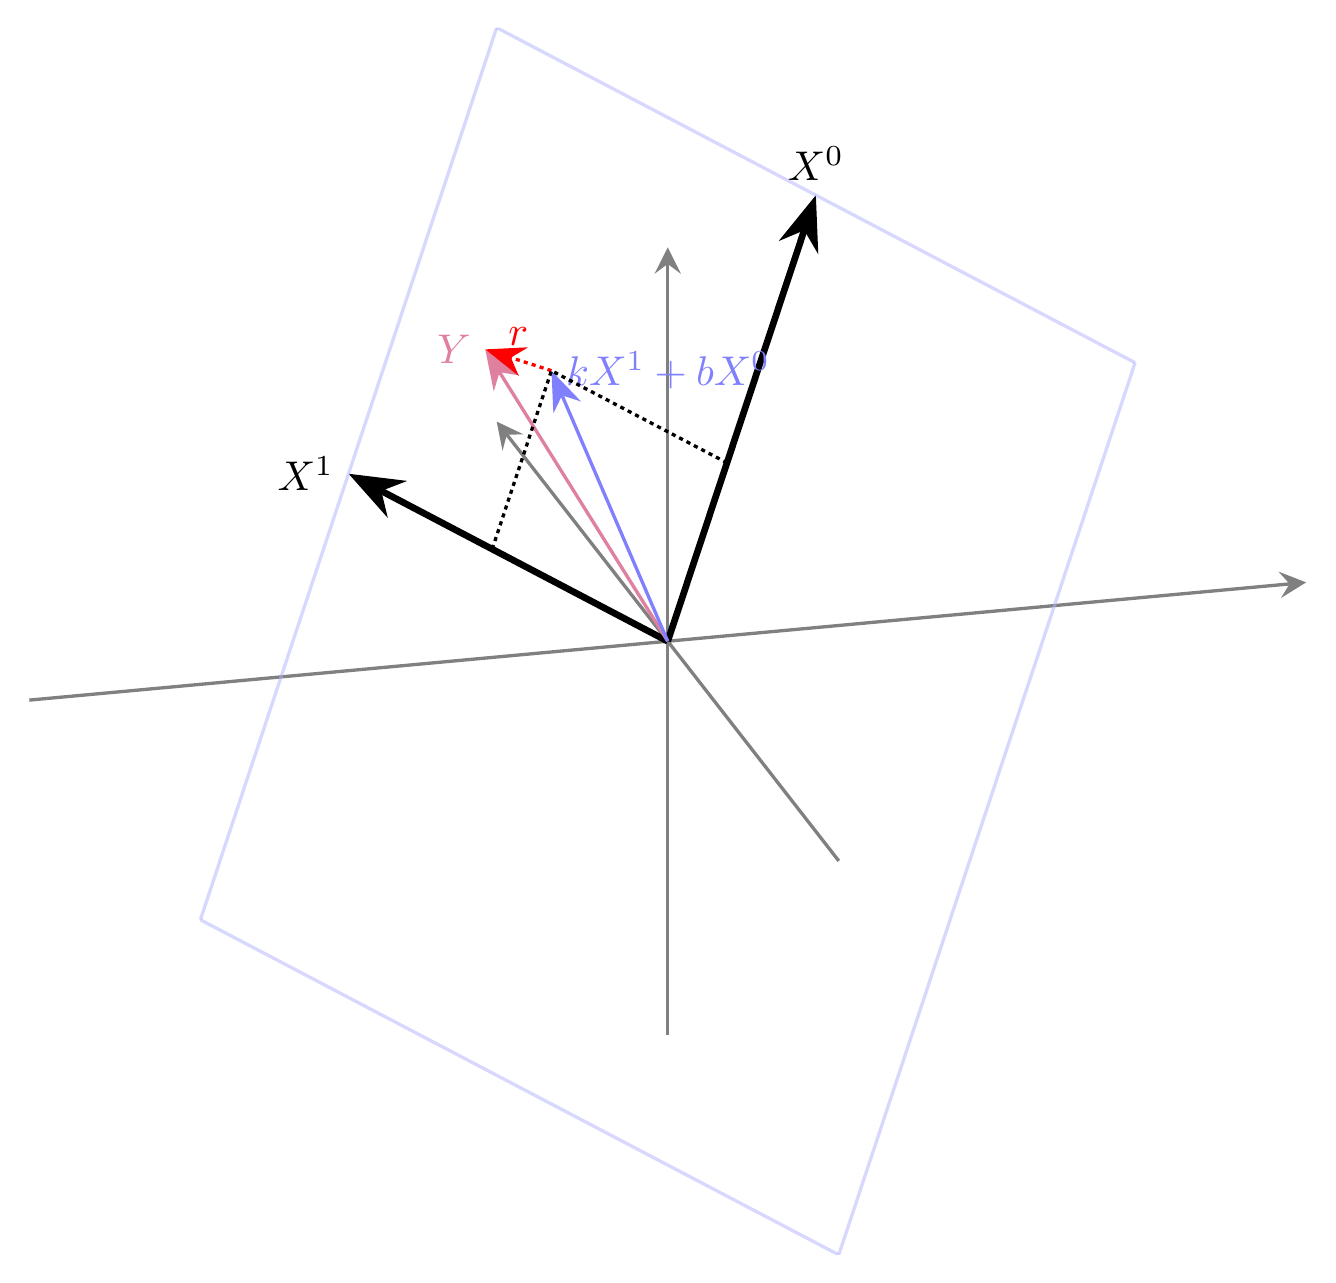
\begin{tikzpicture}[>=Stealth, scale=3]
    \begin{axis}[
            view={-15}{30},      % 设置视角 (方位角, 俯仰角)
            axis lines=center,  % 轴从原点开始
            enlargelimits=false,
            ticks=none,         % 取消刻度
            colormap/viridis,
            axis line style={draw=gray},
            % xlabel={$x$},
            % ylabel={$y$},
            % zlabel={$z$}
        ]

        \coordinate (O) at (axis cs:0,0,0);
        \coordinate (Y) at (axis cs:-0.25, 0.6, 0.85);
        \coordinate (A) at (axis cs:-0.15, 0.4, 0.95);
        
        \addplot3[thick, ->] coordinates {(0,0,0) (1,1,1)} ;
        \node[above, scale=0.5] at (axis cs:1,1,1) {$X^0$};

        \addplot3[thick, ->] coordinates {(0,0,0) (-1,0,1)};
        \node[left, scale=0.5] at (axis cs:-1,0,1) {$X^1$};

        \addplot3[thin, purple!50, ->] coordinates {(0,0,0) (-0.25, 0.6, 0.85)};
        \node[left, purple!50, scale=0.5] at (Y) {$Y$};

        \addplot3[thin, blue!50, ->] coordinates {(0,0,0) (-0.15, 0.4, 0.95)};
        \node[right, blue!50, scale=0.5] at (A) {$kX^1 + bX^0$};

        \addplot3[red, dash pattern=on 0.5pt off 0.5pt, ->] coordinates {(-0.15,0.4,0.95) (-0.25, 0.6, 0.85)};
        \node[red, above, scale=0.5] at (axis cs:-0.2, 0.5, 0.9) {$r$};

        \addplot3[thin, dash pattern=on 0.5pt off 0.5pt] coordinates {(0.4, 0.4, 0.4) (-0.15, 0.4, 0.95) (-0.55, 0, 0.55)};

        \addplot3[surf, color=blue!30, fill=blue!30, shader=flat, opacity=0.5]
        coordinates {(0,1,2) (2,1,0) (0,-1,-2) (-2,-1,0) (0,1,2)};
    \end{axis}
\end{tikzpicture}
\caption{从几何的角度看残差}
\end{figure}

从几何上,$kX^1 + bX^0$ 落在它们所处的平面上,求 $r = Y - (kX^1 + bX^0)$ 的最小值实际上就是从点向平面做垂线并求垂线长。平面上的点恰好表示了那些可以精准拟合的数据,而偏离平面的部分则暗示了无论怎么用直线拟合都会有误差。不得不说从几何上看确实清晰很多,事实上也有人从几何角度给出了\uhref{https://www.bilibili.com/video/BV15zPBevERL}{推导},不过掠过这些细节,仅保留一个直观的印象也无大碍。在本节初的推荐阅读中用不同的方法解答了如何最小化误差,因此这里不再赘述。但是我认为如果读者有一些基础的统计知识而且想记住线性回归推导出的结果,那么结论值得一提,不过跳过也无妨。计算出来的结论是这样的:

首先要计算的是样本中心点,对 $b$ 的导数项为 0 推出最优的直线必然经过样本中心点 $(\bar x, \bar y)$,其中
\[
    \bar x = \frac1n \sum_{i=1}^n x_i, \bar y = \frac1n \sum_{i=1}^n y_i
\]
即均值。

看斜率之前先看看方差和协方差,方差\footnote{此注释写给学过数理统计的读者:此处并非样本方差,样本方差除以的是 $n-1$}的表达式是
\[
    \text{Var}(x) = \frac1n \sum_{i=1}^n (x_i - \bar x)^2
\]
是不是感觉很熟悉?这不就是自变量相对均值的 MSE 吗?而协方差的表达式是
\[
    \text{Cov}(x, y) = \frac1n \sum_{i=1}^n (x_i - \bar x)(y_i - \bar y)
\]
它把方差中的平方项换成了 $x$ 和 $y$ 的交叉项,并由此体现出了相关关系。

接下来计算的是斜率 $k$,它的表达式是
\[
    k = \frac{\sum_{i=1}^n (x_i - \bar x)(y_i - \bar y)}{\sum_{i=1}^n (x_i - \bar x)^2}
\]
看起来有些复杂,但是总结起来其实就是协方差除以自变量的方差,即 $k = \text{Cov}(x, y) / \text{Var}(x)$,如果把协方差看作一种乘法\footnote{此注释写给熟悉线性代数的同学:在\uhref{https://en.wikipedia.org/wiki/Inner_product_space\#Random_variables}{向量空间内积}的意义上这几乎正确},那么 $k = (x\cdot y) / (x\cdot x)$ 看起来确实挺像那么回事的。

这样一来,通过点-斜率式就可以得到最优的直线,那么直线拟合就告一段落了。

\vfill

\subsection{多项式拟合}
\subsection{高维的线性拟合}

\section{逻辑亦数据}
% 从程序执行的视角开始,引入数据是如何编码逻辑的
\subsection{逻辑门}
\subsection{程序是怎么执行起来的}
\subsection{位运算与bit-flag}

\section{神经网络:一个大的函数}
% 从函数拟合的角度引入神经网络
\subsection{知道目标就可以拟合了?}
\subsection{激活函数与非线性}
\subsection{神经网络的训练}
\subsection{如果不知道目标,只知道回报呢?}

\section{泛化性:一个矛盾}
% 从训练集到测试集的泛化性
\subsection{过拟合与欠拟合}
\subsection{网络的大小好像小于训练数据?哪来的泛化性}
\subsection{训练好像被卡住了——香农极限}

\section{你能猜到一句话接下来要说什么?}
% 从信息论的角度引入预测
\subsection{什么是“废话”?}
\subsection{jpeg虽然有损,但为什么说是极其成功的?}
\subsection{熵与压缩}
\subsection{马尔可夫链}

\section{压缩即智能}
% 从压缩的角度引入智能
\subsection{你是如何看出对面的人心情怎么样的?}
\subsection{压缩的极限——区分能力的边界}
\subsection{从母语词汇看对事物的认识}
\subsection{压缩的本质}

\section{潜空间:更适合机器人的编码方式}
% 从压缩的角度引入潜空间
\subsection{潜空间是什么?}
\subsection{高维空间的维数灾难}
\subsection{“空空”的空间的另一面——维数远不是储存能力的极限}

\section{但是,代价是什么:可解释性的地狱}
% 从压缩的角度引入可解释性
\subsection{想想什么是“解释”?}
\subsection{神经网络不能很好地被解释}

\section{再论网络结构} %:全连接、循环神经网络、卷积神经网络、残差链接与transformer}
% 介绍常见的网络结构
\subsection{全连接网络}
\subsection{循环神经网络}
\subsection{卷积神经网络}
\subsection{深度学习与残差链接}
\subsection{transformer}
\subsection{自编码器与扩散模型}
\subsection{仿人的架构——专家模型}

\section{杂谈}
% 一些更有哲学或社会学色彩的问题
\subsection{矩阵式研究——场景与模型的排列组合}
\subsection{AI圈的常见行话}
\subsection{AI——生产力还是毁灭?}
\subsection{新人类与自由意志?}

\end{document}